% =============================================================================
% PRESENTACIÓN CANDIDATURA DOCTORAL - V5 NARRATIVA
% Sistema Híbrido para Predicción de Emisiones de CO2 y CH4
% en la Bioconversión de Residuos con Hermetia illucens
% =============================================================================
% Compilación: bash scripts/compilar-local.sh candidatura
% =============================================================================

\documentclass[aspectratio=169, 11pt]{beamer}

% --- Fuentes (XeLaTeX) ---
\usepackage{tcolorbox}
\usepackage{fontspec}
\setmainfont{TeX Gyre Termes}
\setsansfont{TeX Gyre Heros}
\setmonofont{Latin Modern Mono}

\usepackage[spanish,es-nodecimaldot]{babel}
\usepackage{amsmath, amssymb, amsfonts}
\usepackage{booktabs}
\usepackage{graphicx}
\usepackage[backend=biber,style=numeric,url=true,doi=true,isbn=false,eprint=false]{biblatex}
\addbibresource{referencias.bib}  % o la ruta: ../tesis/referencias.bib
\usepackage{tikz}
\usetikzlibrary{shapes.geometric, arrows.meta, positioning, calc, fit, shadows, shapes.symbols}

% --- Tema y colores ---
\usetheme{Madrid}
\usecolortheme{beaver}
\definecolor{unalRojo}{RGB}{148, 36, 36}
\definecolor{verdeOK}{RGB}{34, 139, 34}
\definecolor{naranjaAlerta}{RGB}{230, 126, 34}
\definecolor{rojoAlerta}{RGB}{192, 57, 43}
\setbeamercolor{structure}{fg=unalRojo}
\setbeamercolor{block title}{bg=unalRojo!15, fg=unalRojo}
\setbeamercolor{block body}{bg=unalRojo!5}
\setbeamercolor{alerted text}{fg=rojoAlerta}

% --- Metadatos ---
\title[Sistema Híbrido BSF]{Sistema Híbrido para Predicción de Emisiones}
\subtitle{CO$_2$ y CH$_4$ en Bioconversión con \textit{Hermetia illucens}}
\author{John Jairo Leal Gómez}
\institute[UNAL]{Doctorado en Estudios Ambientales\\Universidad Nacional de Colombia -- Sede Palmira}
\date{Abril 2026}
\titlegraphic{
\includegraphics[width=1.5cm]{../tesis/00Figuras/00f00EscudoUN2016.jpg}}

% --- Comandos ---
\newcommand{\BSF}{\textit{Hermetia illucens}}
\newcommand{\MAPE}{\text{MAPE}}
\newcommand{\DEB}{\text{DEB}}
\newcommand{\NDIR}{\text{NDIR}}
\newcommand{\MRV}{\text{MRV}}

\setbeamertemplate{navigation symbols}{}
\setbeamertemplate{footline}[frame number]
%\setbeamertemplate{footline}{%
%  \leavevmode%
%  \hbox{%
%  \begin{beamercolorbox}[wd=\paperwidth,ht=2.5ex,dp=1ex,center]{structure}%
%    \usebeamerfont{page number in head/foot}%
%    \insertframenumber{} / \inserttotalframenumber
%  \end{beamercolorbox}}%
%  \vskip0pt%
%}
\begin{document}
% =============================================================================
% 1. PORTADA
% =============================================================================
\begin{frame}[plain]
    \titlepage
\end{frame}
\tableofcontents

% =============================================================================
% 2. SLIDE 2 CONTEXTO
% =============================================================================

% ============================================
% DIAPOSITIVA 2a: GEI - Comparativa histórica
% ============================================
% =============================================================================
% CONTEXTO I: GEI EN ESCALADA — NARRATIVA PROBLEMÁTICA
% =============================================================================
\section{Introducción}
%======================================================================
% BLOQUE: EL PROBLEMA DE LOS RESIDUOS Y EL VACÍO DE TRAZABILIDAD
%======================================================================

%----------------------------------------------------------------------
% Diapositiva 1: El gran problema
%----------------------------------------------------------------------
\begin{frame}{Los residuos org\'{a}nicos como fuente de gases de efecto invernadero}
\begin{columns}[T]
\begin{column}{0.48\textwidth}
\begin{block}{Problema global}
\footnotesize
La fracci\'on org\'anica de los residuos s\'olidos 
constituye una de las fuentes m\'as significativas de 
emisiones antropog\'enicas de metano a escala 
mundial~\cite{fao2021waste,kong2012evaluating}. 
En condiciones de descomposici\'on anaerobia 
---vertederos mal manejados, compostaje deficiente--- 
se generan~\cite{nordahl2023greenhouse}:

\vspace{0.1cm}
\begin{itemize}
    \item \textbf{CO$_2$} (respiraci\'on aerobia)
    \item \textbf{CH$_4$} (metanog\'enesis anaerobia)
    \item \textbf{N$_2$O} (nitrificaci\'on--denitrificaci\'on incompleta)
    \item NH$_3$, compuestos org\'anicos vol\'atiles (olor)
\end{itemize}
\end{block}
\end{column}
\begin{column}{0.48\textwidth}
\begin{exampleblock}{Contexto Colombia}
\footnotesize
El pa\'{i}s ratific\'{o} la meta de reducir \textbf{51\%} de sus emisiones proyectadas al 2030. Los residuos agroindustriales mantienen peso creciente en el perfil nacional de GEI seg\'{u}n el IDEAM \cite{colombia2020ndc,ideam2021inventario}.

\vspace{0.2cm}
\textbf{Vac\'{i}o estructural:} a\'{u}n faltan sistemas de medici\'{o}n continua que permitan saber cu\'{a}nto se emite realmente durante el tratamiento biol\'{o}gico de estos residuos.
\end{exampleblock}
%\vspace{0.2cm}
\begin{alertblock}{Problema central}
\footnotesize
\textit{No se puede mitigar bien lo que no se mide en tiempo real.}
\end{alertblock}
\end{column}
\end{columns}
\end{frame}
%%%%%%%%%%%%%%%%%%%%%%%%%%%%%%%%%%%%%%%%%%%%%%%%%%%%%%%%%%%%%%%%%%%%%%%%%%%%%%%%%%%%%%%%%%%%%%%%%%%%%%%%
\begin{frame}{Contexto: GEI en Escalada --- 50 A\~{n}os de Crecimiento Acelerado}

\begin{block}{La escalada cuantificada (1974 $\rightarrow$ 2024)}
\centering
\begin{tabular}{lccc}
\toprule
\textbf{Gas} & \textbf{1974} & \textbf{2024} & \textbf{Crecimiento} \\
\midrule
CO$_2$  & $\sim$330 ppm  & 423.9 ppm & +28\% \\
\textbf{CH$_4$}  & $\sim$1510 ppb & 1942 ppb  & \textbf{+29\%} \\
N$_2$O  & $\sim$298 ppb  & 338 ppb   & +13\% \\
\bottomrule
\end{tabular}

\vspace{0.2cm}
\footnotesize Fuente: NOAA Global Monitoring Laboratory~\cite{noaa2024ch4} / WMO~\cite{wmo2025}
\end{block}

\vspace{0.2cm}

\begin{alertblock}{Origen y vac\'io}
\footnotesize
La descomposici\'on anaer\'obica de residuos org\'anicos en vertederos sin control 
---especialmente en el Sur Global--- genera $\sim$15--20\% de las emisiones 
antropog\'enicas de CH$_4$, cuyo potencial de calentamiento global es de 
\textbf{80$\times$ en 20 a\~nos} y \textbf{27 a 30$\times$ en 100 a\~nos}~\cite{ipcc2021ar6}. 
A pesar de que CH$_4$ creci\'o un 29\% en cinco d\'ecadas~\cite{wmo2025}, 
su trazabilidad en los procesos de tratamiento biol\'ogico sigue siendo \textbf{nula}.
\end{alertblock}

%\vspace{0.1cm}
\centering
\textit{\footnotesize La escalada demuestra la urgencia, pero las tecnolog\'{i}as de tratamiento a\'{u}n operan sin predicci\'{o}n de emisiones en tiempo real.}

\end{frame}

% =============================================================================
% TECNOLOGIAS DE GESTION DE RESIDUOS ORGANICOS
% =============================================================================
\begin{frame}{Tecnologías de gestión de residuos orgánicos}

\footnotesize
\begin{tabular}{lcccc}
\toprule
\textbf{Tecnología} & \textbf{Tiempo} & \textbf{Riesgo CH$_4$} & \textbf{Productos} & \textbf{Monitoreo} \\
\midrule
Vertedero        & Años     & Alto              & Ninguno                  & Bajo o nulo \\
Compostaje       & Meses    & Medio             & Compost                  & Manual / puntual \\
Biodigestión     & Semanas  & Alto (controlable) & Biogás + digestato      & Parcial \\
\textbf{Bioconversión BSF} & \textbf{Días} & \textbf{Bajo, pero variable} & \textbf{Biomasa + frass} & \textbf{Muy limitado} \\
\bottomrule
\end{tabular}

\vspace{0.25cm}

\begin{columns}[T]
\begin{column}{0.48\textwidth}
\begin{block}{¿Por qué interesa BSF?}
\footnotesize
\begin{itemize}
    \item Proceso rápido de valorización de residuos
    \item Genera biomasa y frass con valor agregado
    \item Puede operar a escalas descentralizadas
    \item Potencialmente menor riesgo de CH$_4$ que rutas anaerobias mal controladas
\end{itemize}
\end{block}
\end{column}

\begin{column}{0.48\textwidth}
\begin{alertblock}{Brecha de conocimiento}
\footnotesize
\begin{itemize}
    \item El desempeño ambiental depende de humedad, aireación y sustrato
    \item Las emisiones no se miden de forma continua
    \item No se detectan en tiempo real eventos críticos de anaerobiosis
\end{itemize}
\end{alertblock}
\end{column}
\end{columns}

\vspace{0.15cm}
\centering
\textit{\footnotesize BSF es prometedora, pero su ventaja climática debe validarse con monitoreo continuo de emisiones.}
\end{frame}
%%%%%%%%%%%%%%%%%%%%%%%%%%%%%%%%%%%%%%%%%%%%%%%%%%%%%%%%%%%%%%%%%%%%%%%%%%%%%%%%%%%%%%%%%%%%%%%%%%%%%%%%%%%%%%%%%%
% =============================================================================
% MARCO TEORICO: TECNOLOGIA, SOCIEDAD Y AMBIENTE
% =============================================================================
\section{Marco teórico}
\begin{frame}{Tecnología, Sociedad y Ambiente}

\begin{block}{Tres dimensiones que convergen}
\footnotesize
\begin{enumerate}
   \item \textbf{Gestión ambiental}: mitigar emisiones exige medirlas 
con trazabilidad y continuidad~\cite{wmo2025,jenkins2025processing,rossi2024estimating}

   \item \textbf{Ciencia y tecnología contextualizada}: los modelos y sensores deben responder a residuos, clima y operación reales del Valle del Cauca~\cite{minciencias2020guia}
\item \textbf{Desarrollo local}: generar datos, código y herramientas propias 
fortalece la autonomía técnica para decidir sobre los residuos~\cite{carolan2020automated,klerkx2019review}

\end{enumerate}
\end{block}

\vspace{0.2cm}

\begin{alertblock}{Postura de la investigación}
\footnotesize
La ausencia de monitoreo continuo no se resuelve solo importando tecnología. Se requiere diseñar infraestructura científica de bajo costo, adaptable y bajo control local, capaz de convertir datos en decisiones para productores, investigadores y gestores del territorio.
\end{alertblock}

\end{frame}
\begin{frame}{BSF: de alternativa prometedora a solución verificable}

\begin{columns}[T]

\begin{column}{0.48\textwidth}
\begin{alertblock}{El círculo del problema}
\footnotesize
\begin{itemize}
    \item Sin medición continua, no hay trazabilidad ambiental robusta
    \item Sin trazabilidad, es difícil comparar BSF con tecnologías convencionales
    \item Sin evidencia confiable, la adopción queda limitada a pilotos o ensayos aislados
    \item Resultado: se frena la transición hacia tratamientos más eficientes y valorización local de residuos
\end{itemize}
\end{alertblock}
\end{column}

\begin{column}{0.48\textwidth}
\begin{block}{La respuesta propuesta}
\footnotesize
\begin{itemize}
    \item Sensores de bajo costo adaptados a condiciones reales
    \item Procesamiento local de datos (\textit{edge computing})
    \item Código abierto y trazabilidad reproducible
    \item Información útil primero para productores, operadores e investigadores del territorio
    \item Generación de métricas de medición ambientales
\end{itemize}
\end{block}
\end{column}

\end{columns}

\vspace{0.3cm}

\centering
\textit{\footnotesize El reto no es solo medir mejor, sino construir capacidad técnica local para interpretar y gestionar ambientalmente los residuos.}

\end{frame}

% =============================================================================
% POR QUE HERMETIA ILLUCENS
% =============================================================================
\begin{frame}{?`Por qu\'e \BSF{} como Agente de Bioconversi\'on?}

\begin{columns}[T]

\begin{column}{0.48\textwidth}
\begin{block}{Capacidades biol\'ogicas excepcionales}
\footnotesize
\begin{itemize}
    \item \textbf{Omn\'ivora extrema}: consume residuos vegetales, animales, fecales, 
          agroindustriales~\cite{singh2019inclusive,bermudez2023comprehensive}
   \item \textbf{Alta Eficiencia}: reduce masa de residuos 50--80\% en 10--14 d\'ias~\cite{singh2019inclusive,surendra2016bioconversion}
    \item \textbf{Crecimiento exponencial}: larva multiplica su peso hasta 
          \textbf{1.000$\times$} en dos semanas~\cite{padmanabha2020comprehensive,eriksen2022dynamic}
    \item \textbf{Resiliente tropical}: tolera 15--40$^\circ$C, ideal para el tr\'opico 
          sin climatizaci\'on costosa~\cite{salam2022effect}
\end{itemize}
\end{block}
\end{column}

\begin{column}{0.48\textwidth}
\begin{block}{Valorizaci\'on total del residuo \cite{bermudez2023comprehensive}}
\footnotesize
\begin{itemize}
    \item \textbf{Biomasa larval}: alto contenido proteico y lip\'idico 
(37--56\% prote\'ina, 14--39\% grasa seg\'un sustrato)
    \item \textbf{Frass}: excretas ricas en N-P-K $\rightarrow$ fertilizante org\'anico de alta calidad    
    \item \textbf{Econom\'ia circular}: biomasa y frass como \'unicos productos finales, 
cerrando el ciclo de nutrientes
    \item \textbf{Seguridad alimentaria}: adultos no pican, no transmiten enfermedades, no son plagas
\end{itemize}
\end{block}
\end{column}

\end{columns}

\vspace{0.3cm}
\centering
\textit{\footnotesize BSF integra, en un mismo sistema, valorización de residuos, producción de biomasa y procesamiento rápido.}

\end{frame}
\begin{frame}%{El Ciclo de Vida de \BSF}
\centering
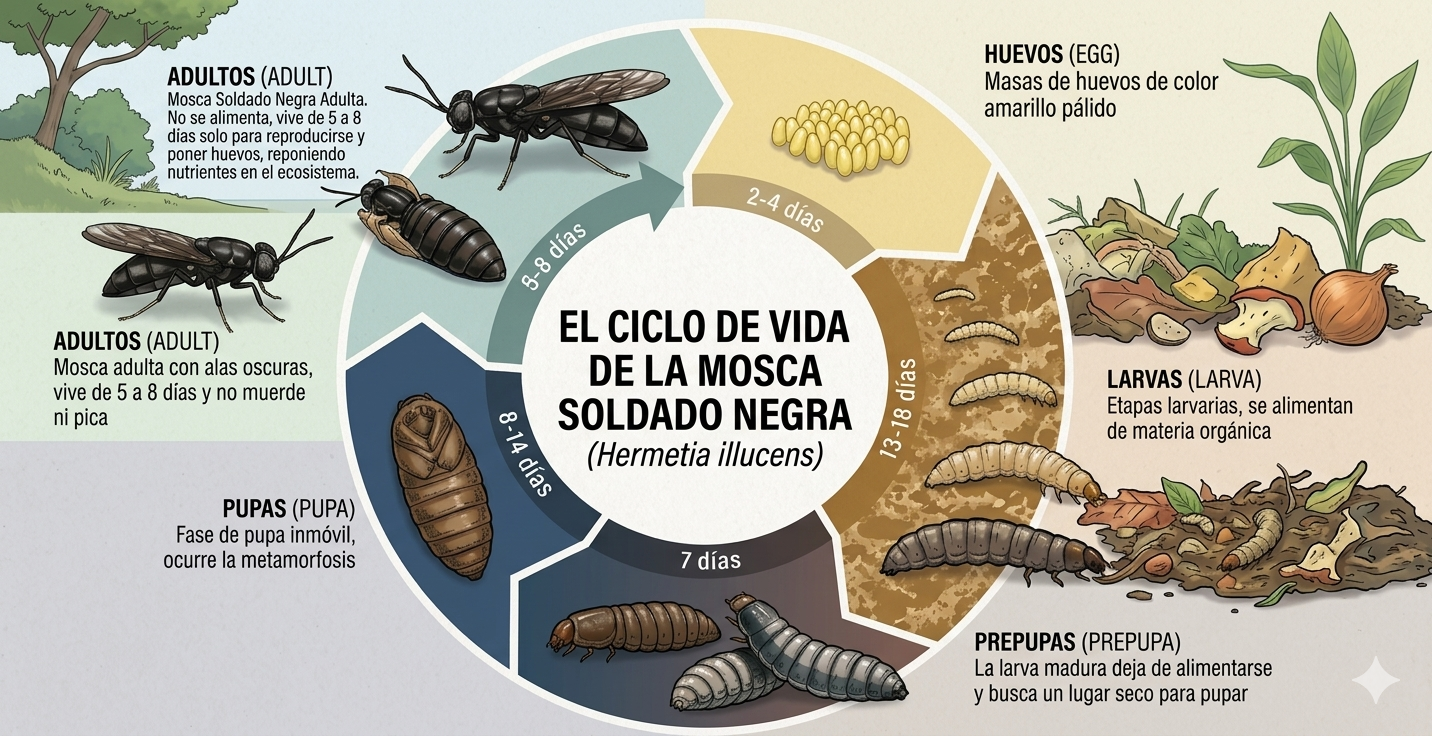
\includegraphics[scale = 0.3]{ciclo-bsf.png}
\par\medskip\footnotesize\textit{Imagen generada por LLM Gemini AI}
\end{frame}
\begin{frame}{}%Etapa larval}
\centering
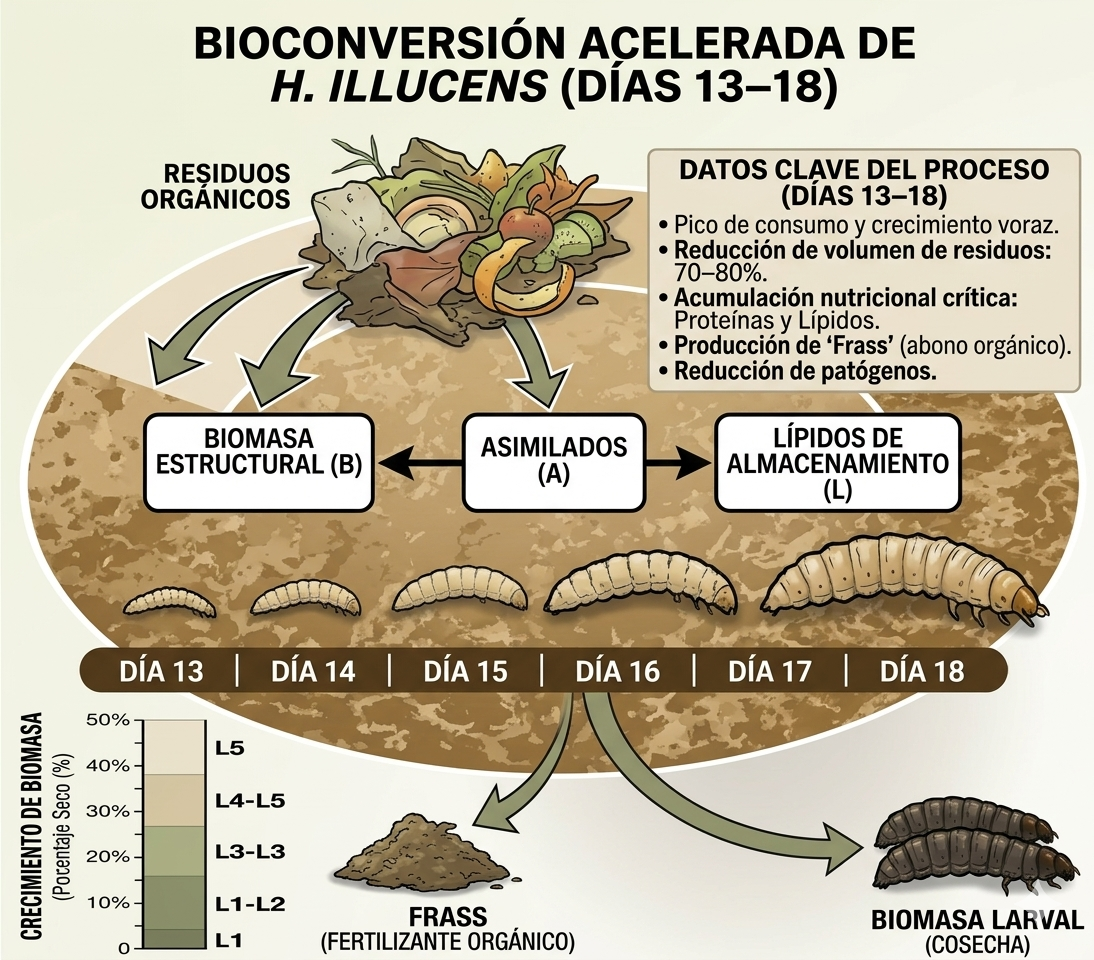
\includegraphics[scale=0.235]{larvas4.png}
\par\medskip\footnotesize\textit{Imagen generada por LLM Gemini AI}
\end{frame}
\begin{frame}
\centering
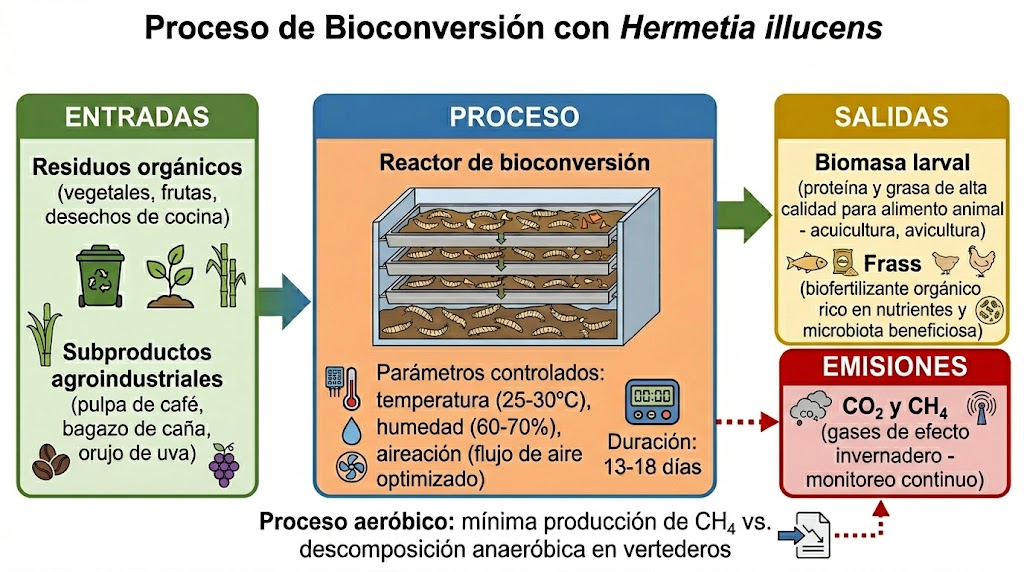
\includegraphics[scale = 0.4]{bioconversion.jpg}
\par\medskip\footnotesize\textit{Imagen generada por LLM Gemini AI}
\end{frame}
%%%%%%%%%%%%%%%%%%%%%%%%%%%%%%%%%%%%%%%%%%%%%%%%%%%%%%%%%%%%%%%%%%%%%%%%%%%%%%
% =============================================================================
% PROCESO DE BIOCONVERSIÓN CON HERMETIA ILLUCENS
% =========================================================================
\section{Proceso de Bioconversión}
\begin{frame}{Bioconversi\'on: De Residuo a Recurso}

\begin{block}{Descripci\'on del proceso}
\footnotesize
\begin{enumerate}
    \item \textbf{Entrada:} Residuos org\'anicos (vegetales, frutas, desechos de cocina) 
    y subproductos agroindustriales (pulpa de caf\'e, bagazo de ca\~na) se introducen 
    en el reactor de bioconversi\'on~\cite{singh2019inclusive,bermudez2023comprehensive}.
    
    \item \textbf{Proceso:} Larvas de \BSF{} consumen los residuos en condiciones controladas:
    \begin{itemize}
        \item Temperatura: 25--30$^\circ$C~\cite{salam2022effect}
        \item Humedad del sustrato: 60--70\%~\cite{bekker2021impact}
        \item Proceso \textbf{aer\'obico}~\cite{diener2009conversion}
        \item Duraci\'on: 10--14 d\'ias~\cite{diener2009conversion,surendra2016bioconversion}
    \end{itemize}
    
    \item \textbf{Salidas:}
    \begin{itemize}
        \item \textbf{Biomasa larval:} prote\'ina animal para alimento de peces y 
        aves~\cite{bermudez2023comprehensive}
        \item \textbf{Frass:} fertilizante org\'anico rico en 
        nutrientes~\cite{bermudez2023comprehensive}
    \end{itemize}
    
    \item \textbf{Emisiones:} CO$_2$ y CH$_4$ generados durante el metabolismo larval --- 
    \textcolor{red}{\textbf{variables a predecir y mitigar}}~\cite{rossi2024estimating,fuhrmann2025comprehensive}.
\end{enumerate}
\end{block}

\vspace{0.3cm}
\centering
\textit{\footnotesize Proceso aer\'obico: m\'inima producci\'on de CH$_4$ vs. \textbf{digesti\'on anaer\'obica} en vertederos.}

\end{frame}
%%%%%%%%%%%%%%%%%%%%%%%%%%%%%%%%%%%%%%%%%%%%%%%%%%%%%%%%%%%%%%%%%%%%%%%%%%%
% =============================================================================
% EL PROBLEMA: OPERAR A CIEGAS
% =============================================================================
\begin{frame}{El problema: un proceso que opera como caja negra}

\begin{alertblock}{Sin predicción en tiempo real...}
\footnotesize
\begin{itemize}
    \item \textbf{Anoxia local} $\rightarrow$ CH$_4$ aumenta sin detección oportuna
    \item \textbf{Biomasa larval desconocida} $\rightarrow$ no se identifica con precisión el momento óptimo de cosecha
    \item \textbf{Prepupa no detectable} $\rightarrow$ se pierde biomasa por migración no anticipada
    \item \textbf{Variables ambientales opacas} $\rightarrow$ temperatura, humedad y aireación no se interpretan dinámicamente
    \item \textbf{Dieta y respiración desacopladas} $\rightarrow$ no se entiende su efecto sobre CO$_2$ y riesgo de anaerobiosis
    \item \textbf{Sin trazabilidad robusta} $\rightarrow$ se limita la validación ambiental y la escalabilidad del sistema
\end{itemize}
\end{alertblock}

\vspace{0.25cm}

\begin{block}{Idea clave}
\centering
\textit{Sin monitoreo continuo, la bioconversión con BSF sigue operando como una caja negra.}
\end{block}

\end{frame}

%%%%%%%%%%%%%%%%%%%%%%%%%%%%%%%%%%%%%%%%%%%%%%%%%%%%%%%%%%%%%%%%%%%%%%%%%%%
% =============================================================================
% IMPLICACIONES DEL VACIO DE MONITOREO
% =============================================================================
% =============================================================================
% EL BLOQUEO COMO CONFIGURACION DE PODER
% =============================================================================

%%%%%%%%%%%%%%%%%%%%%%%%%%%%%%%%%%%%%%%%%%%%%%%%%%%%%%%%%%%%%%%%%%%%%%%%%%%%
% =============================================================================
% MODELO DEB: FLUJOS DE CARBONO EN H. ILLUCENS
% =============================================================================
\section{Flujos de carbono}
\begin{frame}{Metabolismo Larval: Flujos de Carbono}

\centering
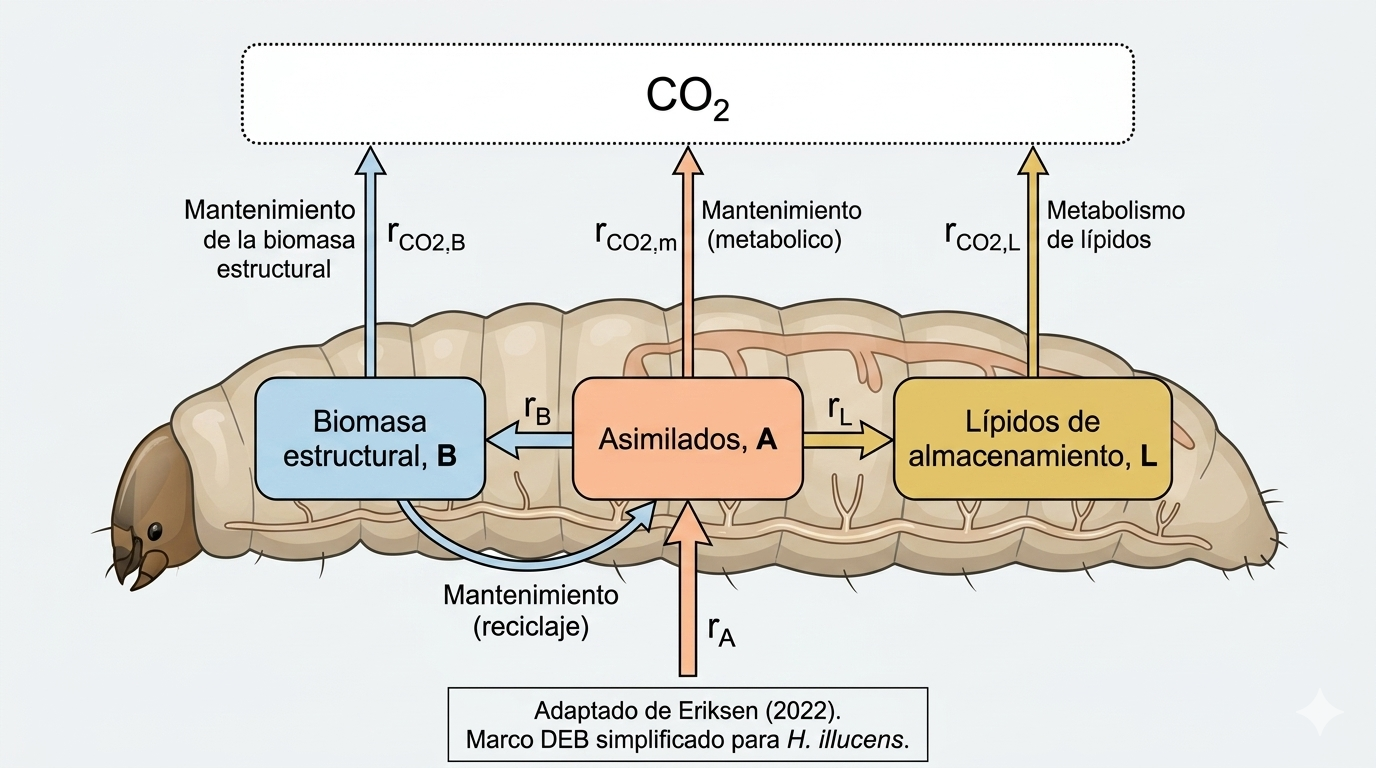
\includegraphics[width=0.84\textwidth]{modelo-deb.png}
\par\medskip\footnotesize\textit{Imagen generada por LLM Gemini AI}

\end{frame}

% =============================================================================
% EXPLICACION DEL MODELO DEB
% =============================================================================
% =============================================================================
% POR QUE EL CO2 ES MEDIBLE: VERSION LIMPIA
% =============================================================================
% =============================================================================
% POR QUE EL CO2 ES MEDIBLE Y MODELABLE
% =============================================================================
\begin{frame}{?`Por qu\'e el CO$_2$ es Medible y Modelable?}

\begin{columns}[T]

\begin{column}{0.48\textwidth}
\begin{block}{El metabolismo larval}
\footnotesize
El carbono asimilado se distribuye en tres reservorios:
\begin{itemize}
    \item \textbf{A (Asimilados):} nutrientes absorbidos del sustrato
    \item \textbf{B (Estructural):} tejidos, m\'usculos, quitina --- lo que se cosecha
    \item \textbf{L (L\'ipidos):} reserva energ\'etica --- calidad de la biomasa
\end{itemize}
\end{block}
\end{column}

\begin{column}{0.48\textwidth}
\begin{alertblock}{La se\~nal CO$_2$}
\footnotesize
Seg\'un el modelo DEB parametrizado para \BSF{} (Eriksen, 2022), entre \textbf{55--60\% del carbono asimilado} se libera como CO$_2$ por respiraci\'on y costos de s\'intesis. Eso lo convierte en un \textbf{proxy cuantitativo} de la actividad biol\'ogica total.

\vspace{0.2cm}
Si el CO$_2$ medido se desv\'ia del modelo DEB:
\begin{itemize}
    \item \textbf{Menor} $\rightarrow$ estr\'es larval, baja ingesta
    \item \textbf{Mayor} + CH$_4$ $\rightarrow$ \textbf{anaerobiosis local}
\end{itemize}
\end{alertblock}
\end{column}

\end{columns}

\end{frame}
%%%%%%%%%%%%%%%%%%%%%%%%%%%%%%%%%%%%%%%%%%%%%%%%%%%%%%%%%%%%%%%%%%%%%%%%%%%%
%%%%%%%%%%%%%%%%%%%%%%%%%%%%%%%%%%%%%%%%%%%%%%%%%%%%%%%%%%%%%%%%%%%%%%%%%%%%%%%%%%%%%%%%%%%%%%%%%%%%%%%%%%%%%%%%%%%%%%%%%%%%%%%%%%%%%%%%%%%%%%%%%%%%%%%%%%%%%%%%%%%%%%%%%%%%%%%%%%%%%%%%%%%%%%%%%%%%%%%%%%%%%%%%%%%%%%%%%%%%%%%%
% =============================================================================
% SLIDE 2: DE LA CAJA NEGRA A LA MEDICION VERIFICABLE
% =============================================================================
\section{Propuesta}
\begin{frame}{De la caja negra a la medición verificable}

\centering
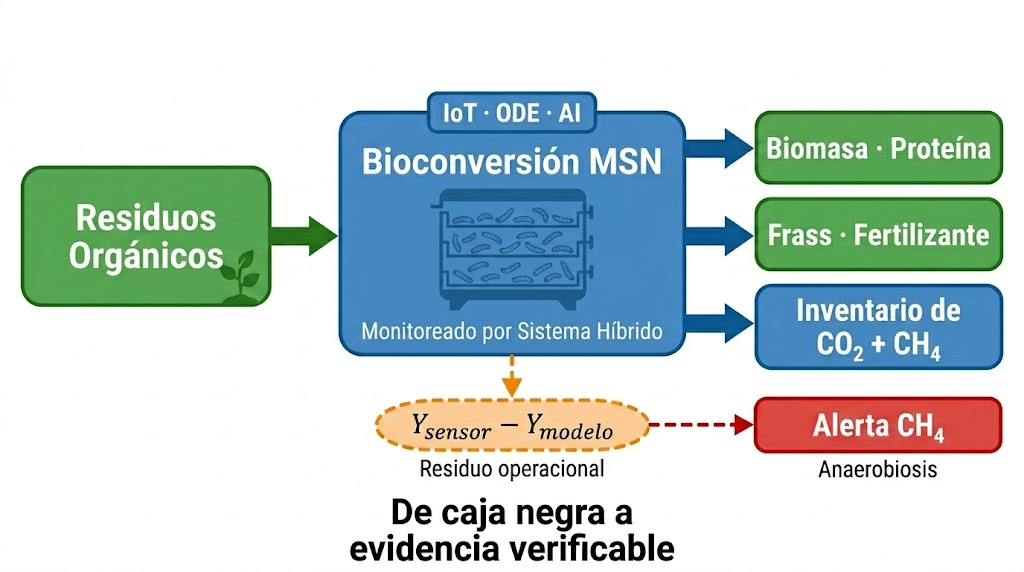
\includegraphics[width=0.83\textwidth]{propuesta.jpg}
\par\medskip\footnotesize\textit{Imagen generada por LLM Gemini AI}
\end{frame}
\begin{frame}{Antecedentes y brecha del sistema híbrido propuesto}

\begin{block}{Estado del arte}
\footnotesize
En \textit{Hermetia illucens}, el estado del arte muestra los siguientes avances principales:
\begin{itemize}
    \item \textbf{Mediciones de GEI:} cuantifican emisiones, pero con muestreos puntuales y metodologías heterogéneas~\cite{rossi2024estimating,fuhrmann2025comprehensive}.
    \item \textbf{Modelos DEB:} describen crecimiento larval y respiración de CO$_2$~\cite{padmanabha2020comprehensive,eriksen2022dynamic}.
    \item \textbf{Monitoreo IoT:} permite seguimiento operativo, aunque sin capacidad predictiva integrada~\cite{raj2023real,duobiene2022development}.
    \item \textbf{Viabilidad ambiental:} La bioconversión con BSF muestra potencial como alternativa de baja emisión frente a rutas convencionales, pero su validación climática sigue limitada por la falta de monitoreo continuo y de factores de emisión específicos~\cite{smetana2019sustainable,jenkins2025processing}.
\end{itemize}
\end{block}

\vspace{0.15cm}

\begin{alertblock}{Brecha que aborda esta tesis}
\footnotesize
Persiste una brecha en la cuantificación dinámica de GEI en sistemas de bioconversión con BSF, lo que impide evaluar con precisión su desempeño ambiental, identificar episodios críticos de anaerobiosis y generar evidencia verificable para estrategias de mitigación.
\end{alertblock}

\end{frame}
% =============================================================================
% DIAPOSITIVA 9: PREGUNTA CENTRAL
% =============================================================================
\begin{frame}{Pregunta de Investigación}
\begin{alertblock}{Pregunta central}
\centering
\large
¿Cómo la integración de un modelo matemático basado en ecuaciones diferenciales ordinarias, sensores IoT de bajo costo y algoritmos de aprendizaje automático permite desarrollar un sistema híbrido que no solo estime con precisión las emisiones de CO$_2$ y CH$_4$, sino que constituya una herramienta de monitoreo dinámico para fundamentar la toma de decisiones operativas y generar métricas verificables del desempeño ambiental en la bioconversión de residuos agroindustriales con \textit{Hermetia illucens}?
\end{alertblock}
\end{frame}

% =============================================================================
% DIAPOSITIVA 10: JUSTIFICACIÓN DE LA PREGUNTA
% =============================================================================
\begin{frame}{Objetivo general}
\begin{block}{Propósito central de la investigación}
\small
Desarrollar un sistema híbrido a escala de laboratorio, integrado por modelado mecanístico basado en EDO, sensores IoT de bajo costo y algoritmos de aprendizaje automático, para estimar la tasa de producción de CO$_2$ y detectar eventos de emisión de CH$_4$ durante la bioconversión de residuos con \textit{Hermetia illucens}, con el fin de generar métricas de desempeño ambiental aplicables a la gestión de residuos agroindustriales.
\end{block}

\end{frame}
% =============================================================================
% OBJETIVOS ESPECIFICOS
% =============================================================================
\begin{frame}{Objetivos espec\'ificos}

\begin{block}{}
\footnotesize
\begin{enumerate}
    \item Diseñar un m\'odulo de sensores NDIR de bajo costo para la medici\'on de CO$_2$ y CH$_4$, determinando su precisi\'on y desviaci\'on (MAPE) frente a un instrumento de referencia bajo condiciones de temperatura y humedad propias del cultivo larval. $\rightarrow$ \textbf{Instrumentaci\'on}

    \item Parametrizar un modelo de EDO basado en la bioenerg\'etica de \textit{Hermetia illucens} para estimar la tasa de respiraci\'on de CO$_2$, evaluando su capacidad predictiva en ventanas temporales durante un ciclo de bioconversi\'on de 15 d\'ias. $\rightarrow$ \textbf{Modelado matem\'atico}

    \item Formular un algoritmo de estimaci\'on de estados, basado en redes neuronales, que infiera la biomasa larval a partir de datos operativos e incorpore esta variable como entrada din\'amica al modelo mecan\'istico para mejorar la precisi\'on de la estimaci\'on de CO$_2$. $\rightarrow$ \textbf{Integraci\'on h\'ibrida}

    \item Validar la utilidad del sistema para la gesti\'on ambiental mediante la detecci\'on de eventos de anaerobiosis asociados a CH$_4$ y la cuantificaci\'on del carbono emitido, contrastando estos indicadores din\'amicos con estimaciones est\'aticas tradicionales. $\rightarrow$ \textbf{M\'etricas ambientales}
\end{enumerate}
\end{block}

\end{frame}%%%%%%%%%%%%%%%%%%%%%%%%%%%%%%%%%%%%%%%%%%%%%%%%%%%%%%%%%%%%%%%%%%%%%%%%%%%%%%%%%%%%%%%%%%%%%%%%%%%%%%%%%%%%%%%%%%
%%%%%%%%%%%%%%%%%%%%%%%%%%%%%%%%%%%%%%%%%%%%%%%%%%%%%%%%%%%%%%%%%%%%%%%%%%%%%%%%%%%%%%%%%%%%%%%%%%%%%%%%%%%%%%%%%%
% =============================================================================
% METODOLOGÍA
% =============================================================================
% =============================================================================
% CONDICIONES AMBIENTALES
% =============================================================================
\begin{frame}{Ubicación y contexto experimental}

\begin{columns}[T,onlytextwidth]
    
    \begin{column}{0.58\textwidth}
        \centering
%        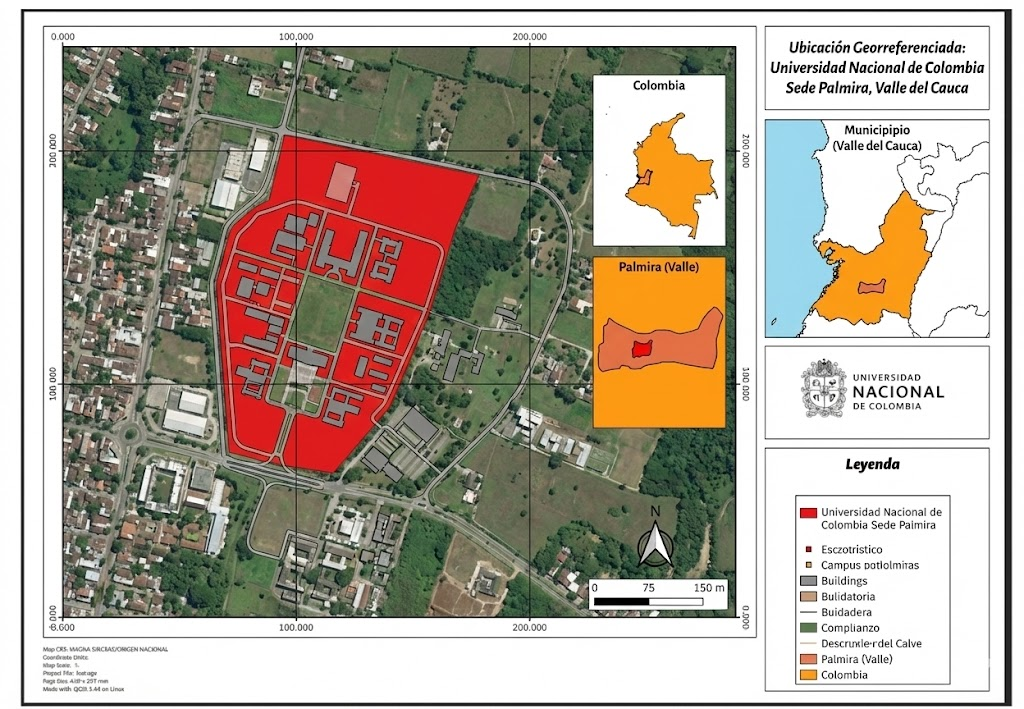
\includegraphics[width=\linewidth]{localizacion.jpg}
        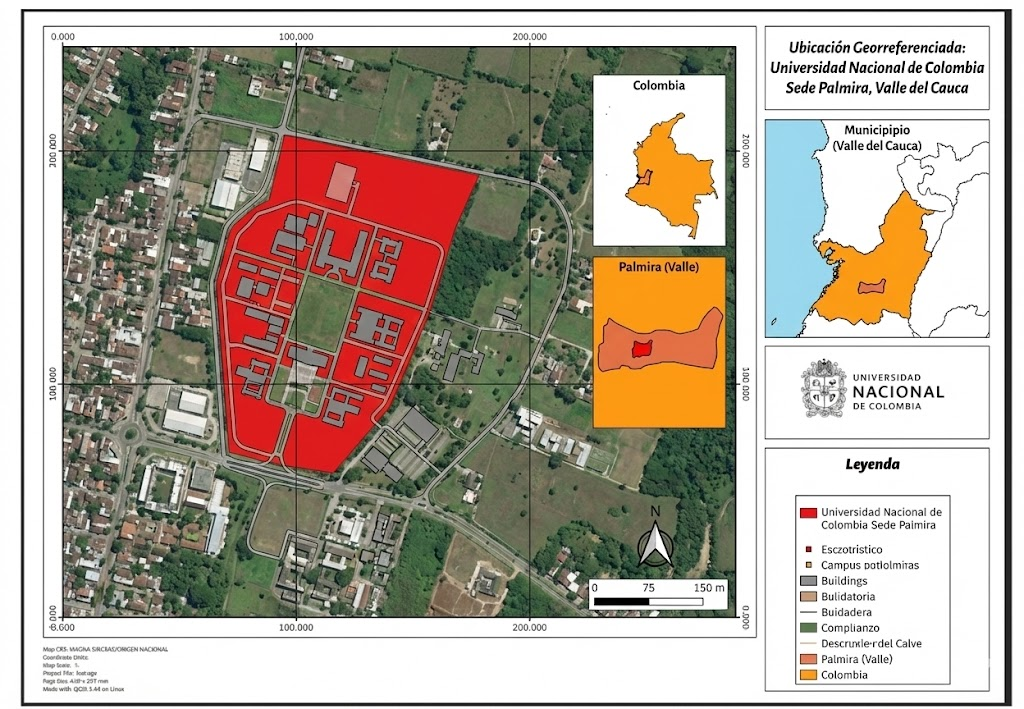
\includegraphics[width=\linewidth,height=0.86\textheight,keepaspectratio]{localizacion.jpg}
    \end{column}
\hspace{0.3cm}
    \begin{column}{0.36\textwidth}
        \begin{block}{Palmira como contexto de estudio}
        \footnotesize
        \begin{itemize}
            \item Altitud media: \textbf{1.001 m s. n. m.}
            \item Temperatura media: $23^oC$
            \item Municipio de vocación \textbf{agroindustrial}
            \item Generación urbana de residuos: \textbf{0,7 kg/hab-día}
            \item Fracción orgánica predominante: \textbf{41,2\%}
        \end{itemize}

        \vspace{0.1cm}
        \footnotesize
        \textbf{Relevancia:} condiciones favorables para estudiar bioconversión de residuos orgánicos y monitoreo ambiental de emisiones.
        \end{block}
    \end{column}

\end{columns}

\end{frame}
% =============================================================================
% METODOLOGÍA
% =============================================================================

\begin{frame}{Marco metodológico}
\framesubtitle{Arquitectura general del sistema}

\begin{columns}[T,onlytextwidth]

\begin{column}{0.48\textwidth}
\begin{block}{Fase I. Adquisición experimental}
\footnotesize
\begin{itemize}
    \item Monitoreo de CO$_2$, CH$_4$, temperatura y humedad
    \item Calibración y validación del módulo sensórico
    \item Construcción del conjunto de datos experimental
\end{itemize}
\end{block}

\vspace{0.2cm}

\begin{block}{Fase II. Modelo mecanístico}
\footnotesize
\begin{itemize}
    \item Formulación bioenergética basada en DEB
    \item Estimación teórica de la respiración aerobia
    \item Definición de una línea base del sistema
\end{itemize}
\end{block}
\end{column}

\begin{column}{0.48\textwidth}
\begin{block}{Fase III. Integración híbrida}
\footnotesize
\begin{itemize}
    \item Inferencia de biomasa mediante redes neuronales
    \item Acople IA + modelo mecanístico
    \item Diagnóstico por contrastación entre medición y predicción
\end{itemize}
\end{block}

\vspace{0.2cm}

\begin{alertblock}{Fase IV. Evaluación ambiental}
\footnotesize
\begin{itemize}
    \item Detección de eventos de anaerobiosis
    \item Estimación dinámica de emisiones
    \item Generación de métricas para apoyo a la gestión
\end{itemize}
\end{alertblock}
\end{column}

\end{columns}

\vspace{0.25cm}
\centering
\footnotesize
\textbf{Secuencia metodológica:} medición $\rightarrow$ modelado $\rightarrow$ integración $\rightarrow$ evaluación
\end{frame}
% =============================================================================
% FASE I
% =============================================================================
\begin{frame}{Fase I: Instrumentación y Aseguramiento de Datos}
\framesubtitle{Del sensor físico al dataset experimental}

\begin{columns}[T,onlytextwidth]

\begin{column}{0.48\textwidth}

\begin{block}{Nodo de medición}
\scriptsize
\begin{itemize}
    \item ESP32 + sensores NDIR (CO$_2$) y electroquímicos (CH$_4$)
    \item Diseño modular: sensor reemplazable, protección ante HR $>80\%$
    \item Resiliencia: buffer SD/Flash + telemetría asíncrona vía MQTT
\end{itemize}
\end{block}

\end{column}

\begin{column}{0.48\textwidth}

\begin{block}{Calibración y validación (H1)}
\scriptsize
\begin{itemize}
    \item Curvas patrón frente a concentraciones certificadas
    \item Compensación cruzada por deriva de temperatura y HR
    \item Criterio de aceptación: $R > 0{,}85$ y MAPE $\leq 15\%$
\end{itemize}
\end{block}

\end{column}

\end{columns}

\vspace{0.20cm}

\begin{alertblock}{Entregable de la Fase I}
\scriptsize
Módulo de sensores calibrado y estable, operando durante ciclos completos de 14--20 días, que genera un \textit{dataset} experimental trazable para alimentar la Fase II (modelo DEB) y la Fase III (RNA).
\end{alertblock}

\vspace{0.15cm}
\centering
\scriptsize
\textbf{Secuencia:} captura confiable $\rightarrow$ calibración robusta $\rightarrow$ dataset estructurado
\end{frame}
% =============================================================================
% FASE II
% =============================================================================
\begin{frame}{Fase II: Modelo Mecanicista de Referencia}
\framesubtitle{Línea base bioenergética DEB para la respiración aeróbica}
\vspace{-0.5cm}
\begin{columns}[T,onlytextwidth]

\begin{column}{0.48\textwidth}

\begin{block}{Fundamento bioenergético}
\scriptsize
\begin{itemize}
    \item EDO simplificado siguiendo el marco DEB para BSF \textcite{eriksen2022dynamic}
    \item La producción de CO$_2$ se desagrega en dos costos acoplados:
    \begin{itemize}
        \scriptsize
        \item \textbf{Mantenimiento:} proporcional a la biomasa actual
        \item \textbf{Biosíntesis:} proporcional a la tasa de crecimiento
    \end{itemize}
    \item Predice la respiración aeróbica del sistema
\end{itemize}
\end{block}

\end{column}

\begin{column}{0.48\textwidth}

\begin{block}{Supuestos y operación}
\scriptsize
\begin{itemize}
    \item \textbf{Aerobiosis estricta:} suministro de O$_2$ ilimitada
    \item \textbf{CH$_4$ excluido:} modelado como perturbación estocástica (zonas anóxicas)
    \item \textbf{Entrada:} biomasa larval $B(t)$ (ajuste logístico o Gompertz)
    \item \textbf{Salida:} curva teórica $Y_{\text{DEB}}$ = ``comportamiento esperado''
\end{itemize}
\end{block}

\end{column}

\end{columns}

\vspace{0.20cm}

\begin{alertblock}{Entregable de la Fase II}
\scriptsize
Ecuaciones de tasa respiratoria parametrizadas para BSF. Se fija un umbral conservador de $R^2 > 0{,}70$, acorde al alcance de un prototipo experimental con sensores de bajo costo, frente a los ajustes $R^2 > 0{,}90$ reportados en modelos dinámicos validados para \textit{H. illucens} en condiciones controladas \parencite{padmanabha2020comprehensive}. Esta línea base sirve como referencia objetiva para contrastar con las mediciones reales en la Fase III.
\end{alertblock}

\vspace{0.15cm}
\centering
\scriptsize
\textbf{Secuencia:} biomasa medida $\rightarrow$ modelo DEB $\rightarrow$ línea base $Y_{\text{DEB}}$ $\rightarrow$ validación cruzada
\end{frame}

% =============================================================================
% FASE III
% =============================================================================

\begin{frame}{Fase III: Integración Híbrida y Validación Cruzada}
\framesubtitle{De la inferencia biológica al diagnóstico operativo}

\begin{columns}[T,onlytextwidth]

\begin{column}{0.48\textwidth}

\begin{block}{Núcleo del sistema híbrido}
\scriptsize
\begin{itemize}
    \item Usar IA como sensor virtual: infiere biomasa larval $B(t)$ a partir de temperatura, HR y señal sensórica
    \item Biomasa discreta (pesaje cada 48 h) se ajusta a curva continua (logística/Gompertz)
    \item Acople IA $\rightarrow$ DEB: la biomasa estimada alimenta el modelo mecanístico
    \item Entrenamiento restringido: la función de pérdida de la RNA incorpora límites bioenergéticos del DEB
\end{itemize}
\end{block}

\end{column}

\begin{column}{0.48\textwidth}

\begin{block}{Contrastación y detección}
\scriptsize
\begin{itemize}
    \item Expectativa teórica $Y_{\text{modelo}}$ vs.\ medición real $Y_{\text{sensor}}$
    \item Residuo operativo:
    \begin{equation*}
        \scriptsize
        Y_{\text{sensor}} = Y_{\text{modelo}} + \delta_{\text{bio}} + \epsilon_{\text{inst}}
    \end{equation*}
    \item Si $|Y_{\text{sensor}} - Y_{\text{modelo}}|$ supera el umbral \textbf{y} correlaciona con CH$_4$, se atribuye a anaerobiosis (zonas anóxicas)
\end{itemize}
\tiny
Donde \quad $Y_{\text{modelo}}$ = predicción DEB, \; $\delta_{\text{bio}}$ = desviación biológica, \; $\epsilon_{\text{inst}}$ = error instrumental

\end{block}

\end{column}

\end{columns}

\vspace{0.20cm}

\begin{alertblock}{Entregable de la Fase III}
\scriptsize
Predictor híbrido (IA $\rightarrow$ DEB) que estima CO$_2$ en tiempo real, detecta eventos de CH$_4$ asociados a anaerobiosis y cuantifica métricas dinámicas de carbono. Éxito: error RMSE inferior al de un modelo de crecimiento lineal estático.
\end{alertblock}

\vspace{0.15cm}
\centering
\scriptsize
\textbf{Secuencia:} biomasa estimada $\rightarrow$ modelo DEB $\rightarrow$ residuo operativo $\rightarrow$ alerta de gestión
\end{frame}

% =============================================================================
% FASE IV
% ============================================================================

\begin{frame}{Fase IV: Métricas Ambientales y Validación Final}
\framesubtitle{Del monitoreo continuo a la gestión verificable}

\begin{columns}[T,onlytextwidth]

\begin{column}{0.48\textwidth}

\begin{block}{Evaluación del desempeño}
\scriptsize
\begin{itemize}
    \item Detección binaria de picos de CH$_4$ donde el modelo predice normalidad (H4)
    \item Criterio: sensibilidad (\textit{Recall}) $> 80\%$ en clasificación de eventos
    \item Tasa temporal de CO$_2$, carbono acumulado y episodios críticos de CH$_4$
    \item Contrastación de métricas dinámicas vs.\ estimaciones estáticas convencionales
\end{itemize}
\end{block}

\end{column}

\begin{column}{0.48\textwidth}

\begin{block}{Interpretación ambiental}
\scriptsize
\begin{itemize}
    \item Discrepancia de masa de CO$_2$: $\Delta_{\text{Total}} = \int_{0}^{t} (Y_{\text{sensor}} - Y_{\text{modelo}})\,dt$
    \item Cuantificación del carbono que el método tradicional no estima
    \item \textbf{Inventario Dinámico de Carbono} (en gramos de C) al final del ciclo
    \item Dato de incertidumbre reducida para reporte ambiental
\end{itemize}
\end{block}

\end{column}

\end{columns}

\vspace{0.20cm}

\begin{alertblock}{Entregable de la Fase IV}
\scriptsize
Sistema validado capaz de detectar anaerobiosis incipiente, explicitar la discrepancia de masa total de CO$_2$ emitida ($\Delta_{\text{Total}}$) y generar reportes consolidados para procesos de Medición, Reporte y Verificación (MRV).
\end{alertblock}

\vspace{0.15cm}
\centering
\scriptsize
\textbf{Secuencia:} evento detectado $\rightarrow$ discrepancia cuantificada $\rightarrow$ alerta operativa $\rightarrow$ reporte MRV
\end{frame}
% =============================================================================
% HIPOTESIS DE TRABAJO
% =============================================================================
\begin{frame}{Matriz de Coherencia: Fases y Criterios de Éxito}
\framesubtitle{Arquitectura en cascada integrada}

\centering
\scriptsize
\renewcommand{\arraystretch}{1.2}
\begin{tabular}{|p{2.6cm}|p{2.8cm}|p{3.8cm}|p{2.8cm}|}
\hline
\textbf{Objetivo} & \textbf{Método / Fase} & \textbf{Entregable Clave} & \textbf{Criterio de Éxito} \\
\hline
1. Instrumentación & Fase I: Adquisición experimental & Módulo de sensores validado en ambiente saturado & $R > 0{,}85$ y MAPE $< 15\%$ (vs.\ referencia) \\
\hline
2. Modelo EDO & Fase II: Modelo Mecanicista & Ecuaciones de tasa respiratoria para \textit{H. illucens} & Capacidad de replicar la tendencia base ($R^2 > 0{,}70$) \\
\hline
3. Integración Híbrida & Fase III: Integración híbrida & Algoritmo de estimación de biomasa y predicción dinámica de CO$_2$ & Error (RMSE) inferior al de un modelo de crecimiento lineal estático \\
\hline
4. Métricas Ambientales & Fase IV: Evaluación ambiental & Inventario Dinámico de Carbono y sistema de alertas & Recall $> 80\%$ en detección de eventos de anaerobiosis (CH$_4$) \\
\hline
\end{tabular}

\vspace{0.25cm}

\begin{columns}[T,onlytextwidth]
\begin{column}{0.48\textwidth}
\centering
\tiny
\textbf{H1:} Precisión instrumental (sensores) \\
\textbf{H2:} Fidelidad bioenergética (modelo DEB)
\end{column}
\begin{column}{0.48\textwidth}
\centering
\tiny
\textbf{H3:} Precisión del sistema híbrido (IA + DEB) \\
\textbf{H4:} Sensibilidad a anomalías (CH$_4$)
\end{column}
\end{columns}

\vspace{0.15cm}
\centering
\tiny
\textit{Encadenamiento lógico: precisión instrumental $\rightarrow$ inferencia de estados $\rightarrow$ fidelidad bioenergética $\rightarrow$ métricas de gestión}
\end{frame}

% =============================================================================
% ALCANCE Y DELIMITACION
% =============================================================================
\begin{frame}{Análisis Crítico I}
\framesubtitle{Materialidad digital, riesgos epistémicos y fronteras del modelo}

\begin{columns}[T,onlytextwidth]

\begin{column}{0.48\textwidth}

\begin{alertblock}{Tensión socioecológica}
\scriptsize
\begin{itemize}
    \item Entorno agresivo (HR $>80\%$, amoniaco, volátiles) acorta vida útil de sensores
    \item Riesgo de \textit{e-waste} y huella de extracción de minerales
    \item Mitigación: arquitectura modular (reemplazar solo sensor, preservar ESP32) y microcontroladores de bajo consumo \parencite{dharCarbonImpactArtificial2020}
\end{itemize}
\end{alertblock}

\vspace{0.12cm}

\begin{block}{Limitaciones estructurales del modelo}
\scriptsize
\begin{itemize}
    \item Especificidad del sustrato: generalización acotada a matrices representadas en el entrenamiento
    \item Resolución 0D temporal: no resuelve gradientes internos de temperatura y oxígeno
    \item Régimen batch: transferencia a sistemas continuos requeriría ajustes
\end{itemize}
\end{block}

\end{column}

\begin{column}{0.48\textwidth}

\begin{alertblock}{Riesgos epistémicos}
\scriptsize
\begin{itemize}
    \item Sobreajuste a condiciones controladas del prototipo
    \item Pérdida de robustez ante variabilidad real de sustratos y microclimas
    \item Predicciones no realistas si la IA opera sin restricciones físicas
\end{itemize}
\end{alertblock}

\vspace{0.12cm}

\begin{block}{Estrategia: IA explicable (XAI)}
\scriptsize
\begin{itemize}
    \item Integración con DEB impone restricciones biológicas en la función de pérdida
    \item Evita tasas de crecimiento negativas o emisiones superiores al carbono disponible
    \item Define \textbf{dónde} el modelo es confiable y \textbf{dónde} requiere recalibración
\end{itemize}
\end{block}

\end{column}

\end{columns}
\end{frame}
\begin{frame}{Análisis Crítico II}
\framesubtitle{Brecha digital, bioseguridad e integridad MRV}

\begin{columns}[T,onlytextwidth]

\begin{column}{0.48\textwidth}

\begin{alertblock}{Retos de escalamiento rural}
\scriptsize
\begin{itemize}
    \item Conectividad inestable o nula (\textit{zonas grises}) excluye arquitecturas centralizadas en nube
    \item Dependencia de soporte técnico especializado como barrera de adopción
\end{itemize}
\end{alertblock}

\vspace{0.12cm}

\begin{block}{Oportunidad: edge computing}
\scriptsize
\begin{itemize}
    \item Algoritmos críticos ejecutados directamente en el nodo ESP32
    \item Operación autónoma y sincronización asíncrona de datos
    \item Costo marginal para pequeños y medianos productores agroindustriales
\end{itemize}
\end{block}

\end{column}

\begin{column}{0.48\textwidth}

\begin{block}{Bioseguridad}
\scriptsize
\begin{itemize}
    \item Detección temprana de anomalías ambientales (fugas, cambios térmicos súbitos)
    \item Alertas para intervención manual inmediata
    \item Apoyo al cumplimiento de normativas fitosanitarias (ICA/UE)
\end{itemize}
\end{block}

\vspace{0.12cm}

\begin{alertblock}{Integridad MRV}
\scriptsize
\begin{itemize}
    \item Trazabilidad digital y \textit{timestamping} de registros de emisiones
    \item Datos auditables bajo estándares IPCC y Verra
    \item Mitiga \textit{greenwashing} digital y sienta bases para certificación de créditos de carbono
\end{itemize}
\end{alertblock}

\end{column}

\end{columns}
\end{frame}
% =============================================================================
% ESTADO ACTUAL (CORREGIDA: sin columnas p{} problemáticas)
% =============================================================================
\section{Estado actual del Proyecto}
\begin{frame}{Estado Actual del Proyecto}

\footnotesize
\begin{tabular}{@{}lll@{}}
\toprule
\textbf{Dimensi\'on} & \textbf{Logros} & \textbf{Estado} \\
\midrule
Te\'orico & Revisi\'on bibliogr\'afica sistematizada. Marco DEB adaptado a BSF. & Completado \\
\addlinespace
Experimental & Mesocosmos operativo (Sede Palmira). Primeros ciclos con CO$_2$ continuo. & En progreso \\
\addlinespace
Computacional & Backend funcional (Node.js, PostgreSQL, MQTT). RNA inicial. & En progreso \\
\bottomrule
\end{tabular}

\vspace{0.4cm}
\centering
\textit{\footnotesize Componentes individuales validados. Desaf\'io actual: integraci\'on conjunta.}

\end{frame}
% =============================================================================
% CRONOGRAMA
% =============================================================================
\begin{frame}{Cronograma: 42 Meses (2023--2027)}
\vspace{-0.5cm}
\centering
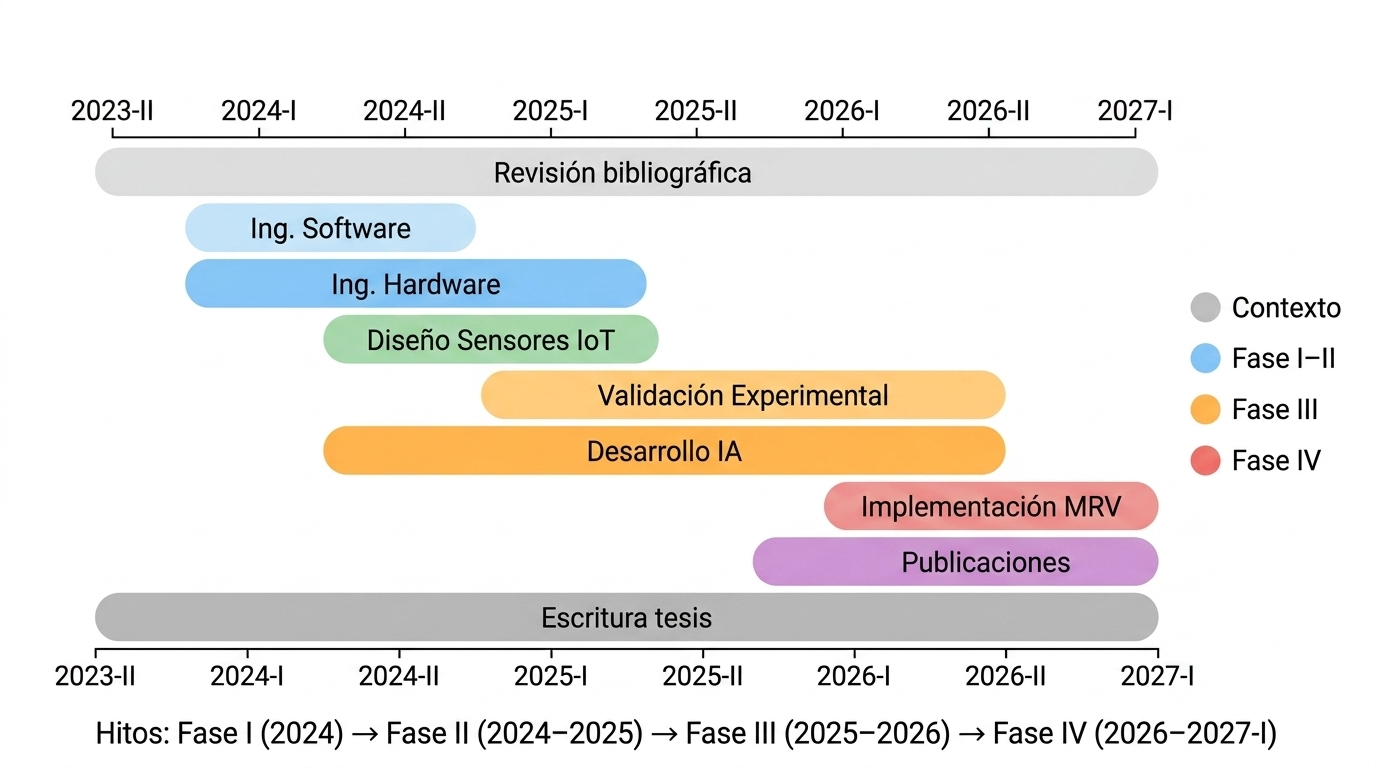
\includegraphics[width=0.85\textwidth]{cronograma.png}
\end{frame}
%%%%%%%%%%%%%%%%%%%%%%%%%%%%%%%%%%%%%%%%%%%%%%%%%%%%%%%%%%%%%%%%%%%%%%%%%%%%%%%%%%%%%%%%%%%%%%%%%%%
% =============================================================================
% CIERRE
% =============================================================================
\section{Cierre}
\begin{frame}{Cierre}

\centering
\Large
\textit{Esta investigaci\'on no propone una tecnolog\'ia perfecta.}

\vspace{0.4cm}

\large
Propone un paso necesario:

\vspace{0.3cm}

\textit{transformar la bioconversi\'on con \BSF{} de una caja negra biol\'ogica}

\vspace{0.1cm}

\textit{en un proceso con \textbf{trazabilidad ambiental}.}

\vspace{0.5cm}

\normalsize
Si los residuos org\'anicos del Sur Global van a ser parte de la soluci\'on clim\'atica,

necesitan dejar de ser parte de la contabilidad incierta.

\end{frame}
% =============================================================================
% GRACIAS
% =============================================================================
\begin{frame}[plain]

\centering
\vspace{2cm}

{\Huge \textbf{Gracias}}

\vspace{1.5cm}

{\large John Jairo Leal G\'omez}

\vspace{0.3cm}

\texttt{jlealgom@unal.edu.co}

\vspace{0.3cm}

Doctorado en Estudios Ambientales

Universidad Nacional de Colombia -- Sede Palmira

\vspace{1cm}

\footnotesize
\textit{``La ausencia de monitoreo no es un rezago tecnol\'ogico:}

\textit{es una configuraci\'on de poder que se resuelve dise\~nando}

\textit{tecnolog\'ia contextualizada, de bajo costo y bajo control local.''}

\end{frame}

%%%%%%%%%%%%%%%%%%%%%%%%%%%%%%%%%%%%%%%%%%%%%%%%%%%%%%%%%%%%%%%%%%%%%%%%%%%%%%%%%%%%%%%%%%%%%%%%%%%%
% =============================================================================
% DIAPOSITIVA DE REFERENCIAS
% =============================================================================
\begin{frame}[allowframebreaks]{Referencias}
\footnotesize
\printbibliography
\end{frame}
\end{document}
